% (C) Marc Lijour, 2019 
% Licensed under a Creative Commons License BY-SA
% https://creativecommons.org/licenses/by-sa/2.5/ca/
% Presentation for Entrepreneurs at Denton's organized by the Lozard Institute
% Hands-on Introduction to Blockchain
% 
% Variables
% TODO set the variables
% ---------------------- USER-DEFINED --------------------------------
\newcommand{\Metameshtitle}{Blockchain~Peer~Group}
\newcommand{\Metameshlongtitle}{A gentle introduction to Blockchain}
\newcommand{\Metameshsubtitle}{at the TechConnex Blockchain Peer Group}
\newcommand{\Metameshauthor}{Marc~Lijour}
\newcommand{\Metameshdate}{February~28, 2019}
\newcommand{\Metameshsubject}{TechConnex}
% --------------------------------------------------------------------
% Template
% (C) Marc Lijour, 2019
% This document is licensed under a Creative Commons License BY-SA (feel free to use the code, but all rights are reserved for logos and art)
% https://creativecommons.org/licenses/by-sa/2.5/ca/
% Metamesh presentation template in LaTeX
% This template comes with a first page on a picture background
% Possible improvement in future iterations
% - Test and fix as needed to work on xetex (to use Ubuntu fonts)
% === USAGE===
% Create a file for your LaTeX content (slides, etc), in which you must do the following:
% TODO 1 - set variables defined below
% TODO 2 - include this code by calling: \input{<the name of this document>}
% TODO 3 - Start the document as usual and you're in business; just use \begin{document} and don't forget to conclude with \end{document}
% TODO 4 - Use the custom method \Metameshcoverpage instead of \titlepage to create your cover page
% Voilà!
%
\documentclass[utf8]{beamer}
\usepackage{etoolbox}
%\usepackage[american,french]{babel}
%\usepackage[T1]{fontenc}
%\usepackage[utf8]{inputenc}
% Variables
% ---------------------- USER-DEFINED --------------------------------
\ifdef{\Metameshtitle}{}{\newcommand{\Metameshtitle}{\color{red}Title TBD}}
\ifdef{\Metameshlongtitle}{}{\newcommand{\Metameshlongtitle}{\color{red}Long title TBD}}
\ifdef{\Metameshsubtitle}{}{\newcommand{\Metameshsubtitle}{\color{red}Subtitle TBD}}
\ifdef{\Metameshauthor}{}{\newcommand{\Metameshauthor}{\color{red}Author TBD}}
\ifdef{\Metameshdate}{}{\newcommand{\Metameshdate}{\color{red}Date TBD}}
\ifdef{\Metameshsubject}{}{\newcommand{\Metameshsubject}{\color{red}Subject TBD}}
% --------------------------------------------------------------------
\usetheme{Boadilla}
% Set color close to Metamesh paletter
%\definecolor{beamer@blendedblue}{RGB}{150,36,36}
%\definecolor{beamer@blendedblue}{RGB}{47,57,118} % dark blue
\definecolor{beamer@blendedblue}{RGB}{75,56,0} % Metamesh colour (yellow)
%\definecolor{beamer@blendedblue}{RGB}{0, 0, 0} % black
% Cover Page
\title[\Metameshtitle] {\Metameshlongtitle}
\subtitle{\Metameshsubtitle}
\author{\Metameshauthor}
\date{\Metameshdate}
\subject{\Metameshsubject}
\usepackage{tikz}
% Try Xetex to use system fonts (pdflatex makes it hard to import a font)
%\usepackage{fontspec}
%\setsansfont{Ubuntu}
%\setmonofont{Ubuntu Mono}

% -- create a custom (command) title page -which has the benefit of not affecting the settings for the rest of the presentation
\newcommand{\Metameshcoverpage}{\frame[plain]{
	\tikz[remember picture,overlay] {
        	\node(bkgd) at ([xshift=0cm,yshift=0cm]current page.center) 
			{
\includegraphics[width=\paperwidth, height=\paperheight]{../../Metamesh-LaTeX_Templates/images/bkg-plain-black}};
		% two logos side by side 
        	\node(logo) at ([xshift=-4cm,yshift=2.7cm]current page.center) 
		 	{
\includegraphics[scale=.5]{../../pics/logos/techconnex-logo}};
        	\node(logo) at ([xshift=4cm,yshift=2.7cm]current page.center) 
		 	{
\includegraphics[scale=.1]{../../Metamesh-LaTeX_Templates/images/logo-white}};
        	\node(CC-BY-SA) at ([xshift=5cm,yshift=-4cm]current page.center) 
			{\href{https://creativecommons.org/licenses/by-sa/2.5/ca/}{
\includegraphics[scale=.4]{../../Metamesh-LaTeX_Templates/images/CC-BY-SA-403x141}}};
	}
	\tikz[remember picture,overlay] {
        	\node(title) at ([xshift=0cm,yshift=0cm]current page.center) 
			%{\Large\color{black}\textbf{{\Metameshlongtitle}}};
			%{\Large\color{beamer@blendedblue}\textbf{{\Metameshlongtitle}}};
			{\Large\color{white}\textbf{{\Metameshlongtitle}}};
        	\node(subtitle) at ([xshift=0cm,yshift=-.7cm]current page.center) 
			%{\small\color{beamer@blendedblue}\emph{\Metameshsubtitle}};
			{\small\color{white}\emph{\Metameshsubtitle}};
        	\node(author) at ([xshift=0cm,yshift=-2cm]current page.center) 
			%{\small\color{beamer@blendedblue}By~\Metameshauthor};
			{\small\color{white}By~\Metameshauthor};
        	\node(date) at ([xshift=0cm,yshift=-2.5cm]current page.center) 
			%{\tiny\color{beamer@blendedblue}\Metameshdate};
			{\tiny\color{white}\Metameshdate};
        	\node(footnote) at ([xshift=0cm,yshift=-3.9cm]current page.center) 
			%{\TINY\color{beamer@blendedblue}\emph{The Art and Science of Eternal Blossom}};
			{\TINY\color{white}\emph{Metamesh Group, your Trusted Advisors for Technology Transformation across the globe}};
        	%\node(footnote) at ([xshift=0cm,yshift=-4.1cm]current page.center) 
		%	{\TINY\color{black}\emph{focusing on Blockchain and related technologies}};
    	}
}}
%
% This sets the ColliderX logo at the bottom right corner of each page
\logo{
	
\includegraphics[scale=.05]{../../Metamesh-LaTeX_Templates/images/logo-black}
}
\AtBeginSection[]
{
  \begin{frame}
    \frametitle{Table of Contents}
    \tableofcontents[currentsection]
  \end{frame}
}
%\usepackage{newunicodechar}
%\usepackage[format=plain,justification=raggedright,singlelinecheck=false]{caption}
\usepackage[format=plain,justification=justified,singlelinecheck=false]{caption} % use this in document to remove "figure": 
%	\captionsetup{labelformat=empty}\caption{caption content} 
% or
% 	\caption*{caption content here}
\usepackage{dirtytalk}
\usepackage{wrapfig}
\usepackage{hyperref}
\usepackage{verbatim}
\usepackage{mathabx}
%\usepackage{MnSymbol}
\usepackage{fancyvrb}


% Extra packages
\usepackage{amssymb}
\usepackage{amsmath}
\usepackage[american]{babel}
\usepackage{csquotes}
\usepackage[backend=biber,style=apa]{biblatex}
\DeclareLanguageMapping{american}{american-apa}
% Use one bib file per section
\addbibresource{references.bib}
\addbibresource{references-ethereum-history.bib}
\definecolor{links}{HTML}{2A1B81}
\hypersetup{colorlinks,linkcolor=,urlcolor=links}
\AtBeginBibliography{\footnotesize}
% Start of the document
\begin{document}
% Cover page
% Do not use this: \frame{\titlepage}
% use this instead:
\Metameshcoverpage

% Content
% (C) Marc Lijour, 2019 
% Licensed under a Creative Commons License BY-SA
% https://creativecommons.org/licenses/by-sa/2.5/ca/
% Presentation for the TechConnex Blockchain Peer Group
% Session 1: Hands-on Introduction to Blockchain
% Presentation touching upon:
% - What is blockchain
% - Hand-on introduction to “crypto” (digital currency, tokens, wallets)
% 
\frame{
	\frametitle{The Blockchain Peer Group is brought to you by}
	\begin{figure}
		
\includegraphics[width=6cm]{../../Metamesh-LaTeX_Templates/images/logo-black}
	\end{figure}
	\center\Large
	\vspace{-2em}
	\href{https://www.metameshgroup.com}{www.metameshgroup.com}
	
}

\frame{
	\frametitle{Who am I?}
	\framesubtitle{\url{https://www.linkedin.com/in/marclijour/}}
	\begin{columns}
	\column{0.3\textwidth}
		\begin{figure}
		
\includegraphics[width=2cm]{../pics/logos/colliderx_logo}
		\end{figure}
	\column{0.3\textwidth}
		\begin{figure}
		
\includegraphics[width=3.5cm]{../pics/logos/consensys-logo-v-630x581}
		\end{figure}
	\column{0.3\textwidth}
		\begin{figure}
		
\includegraphics[width=3cm]{../../Metamesh-LaTeX_Templates/images/logo-black}
		\end{figure}
	\end{columns}
}

\frame{
	\frametitle{Team Experience}
	\begin{figure}
		\includegraphics[width=11cm]{../pics/Metamesh/metamesh-team-experience}
	\end{figure}
}

\frame{
	\frametitle{Access these slides}
	\center\Huge 
	\url{https://bit.ly/2Tou0Jy}\\ 
	\vspace{2em}
	{\normalsize 
		or find in the folder \href{https://bit.ly/2XtRJYb}{2019 TechConnex - Blockchain Peer Group} at\\
		\url{https://github.com/marclijour/presentations}
	}
}

% ======================================================================================================
%                         Introduction to the presentation and What is Blockchain 
% ======================================================================================================
\section{What is Blockchain?}
\frame{
	\frametitle{The Trust Machine}
	\begin{figure}
		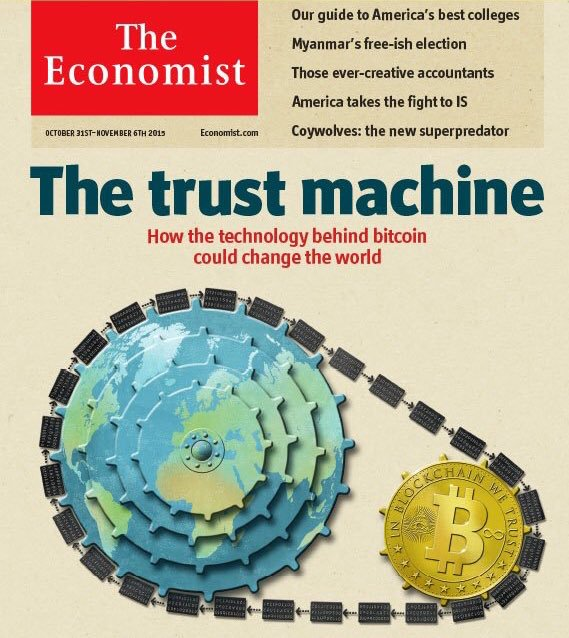
\includegraphics[height=6cm]{../pics/blockchain/economist-trust-machine}
	\end{figure}
}

\frame{
	\frametitle{Source of Trust}
	\framesubtitle{\href{https://www.youtube.com/watch?v=6WG7D47tGb0}{World Economic Forum: \textit{What is Blockchain} Youtube Video}}
	\begin{figure}
		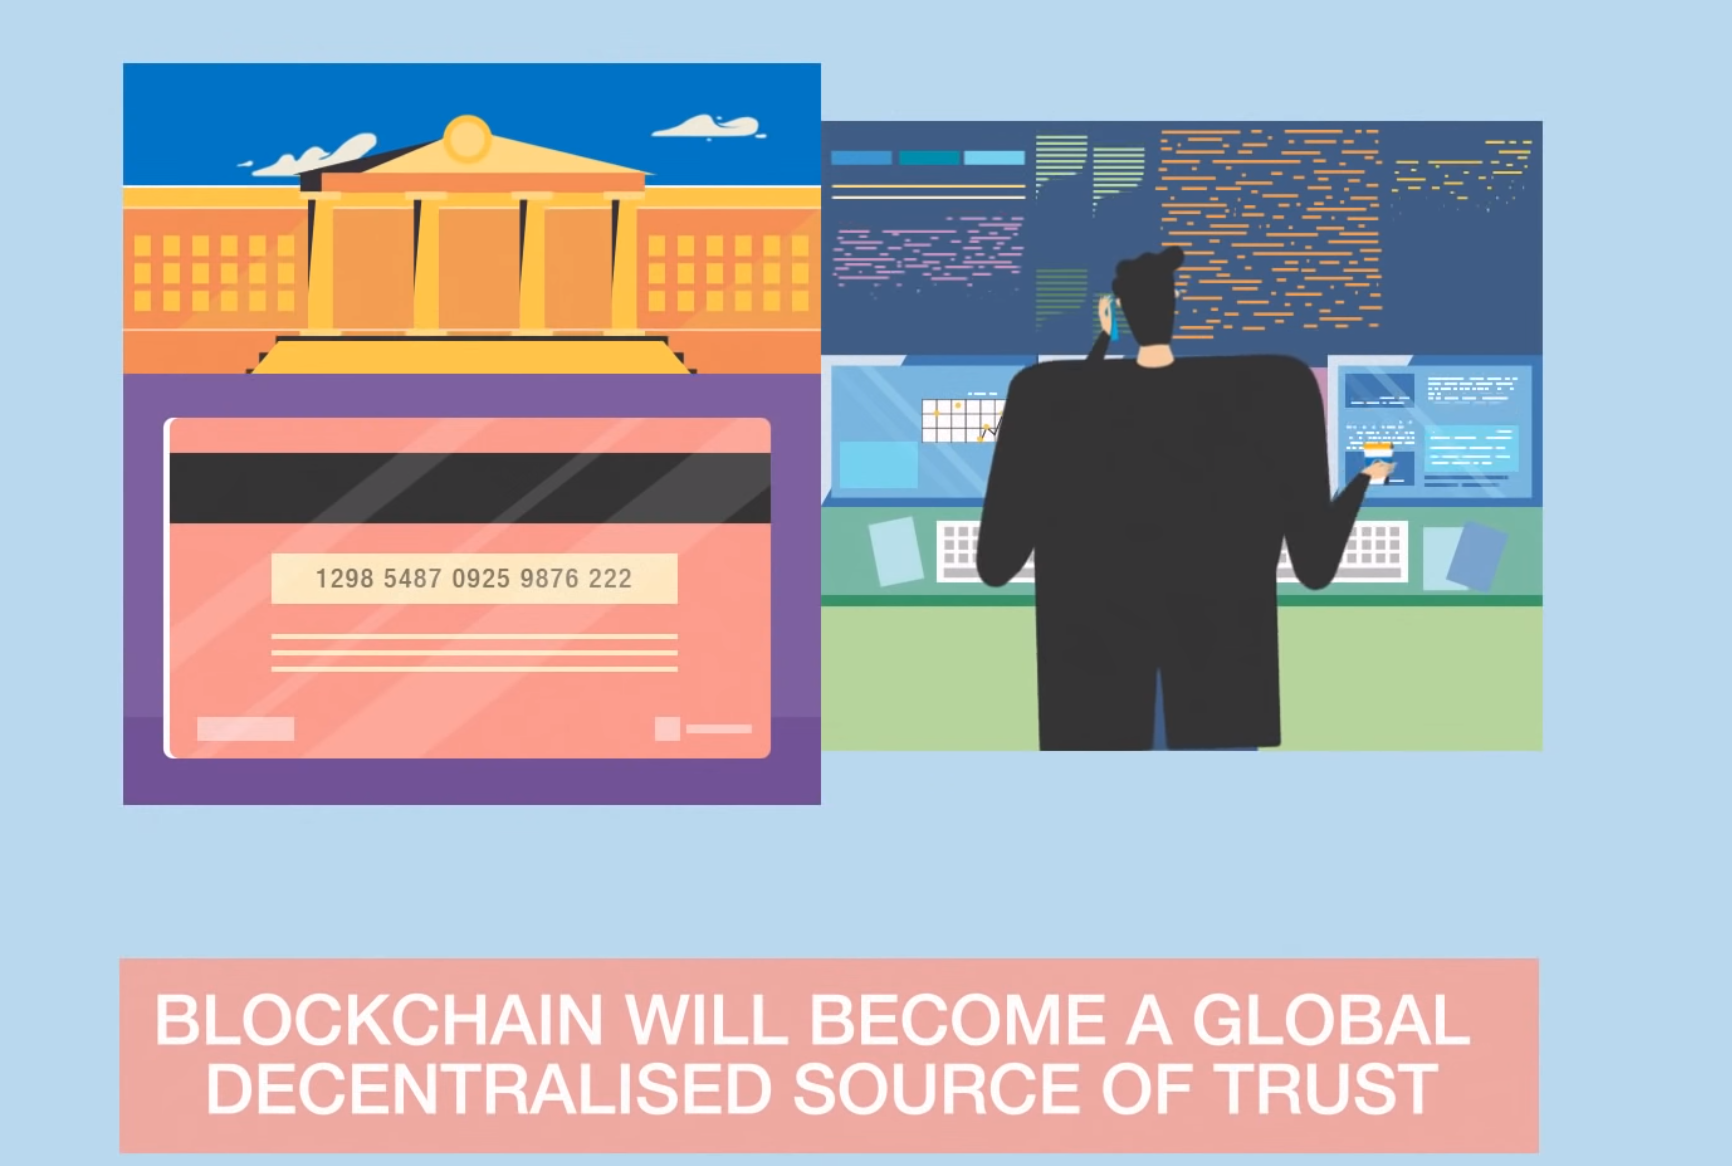
\includegraphics[width=11cm]{../pics/blockchain/wef-blockchain-source-of-trust}
	\end{figure}
}

\frame{
	\frametitle{Key Cryptographic Primitives}
	\begin{columns}[T]
	\column{0.3\textwidth}
		\centering \textbf{Signing}
		\begin{figure}
		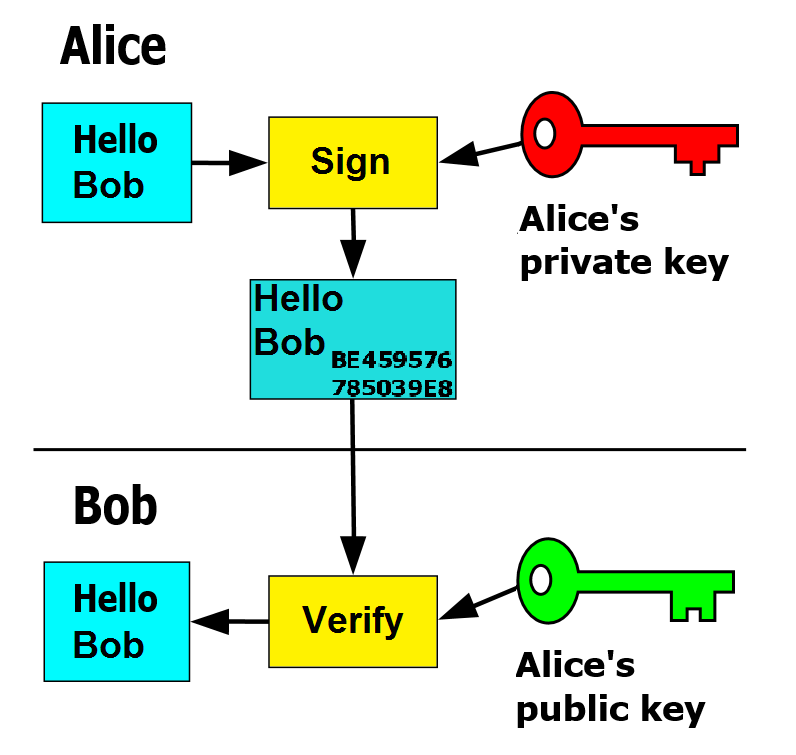
\includegraphics[width=3cm]{../pics/cryptography/Private_key_signing}
		\\
		% CC-BY-SA
		\tiny{Credit: \href{https://commons.wikimedia.org/wiki/User:FlippyFlink}{FlippyFlink}}
		\end{figure}
	\column{0.3\textwidth}
		\centering \textbf{Encrypting}
		\begin{figure}
		% https://en.wikipedia.org/wiki/File:Public_key_encryption.svg
		% public domain
		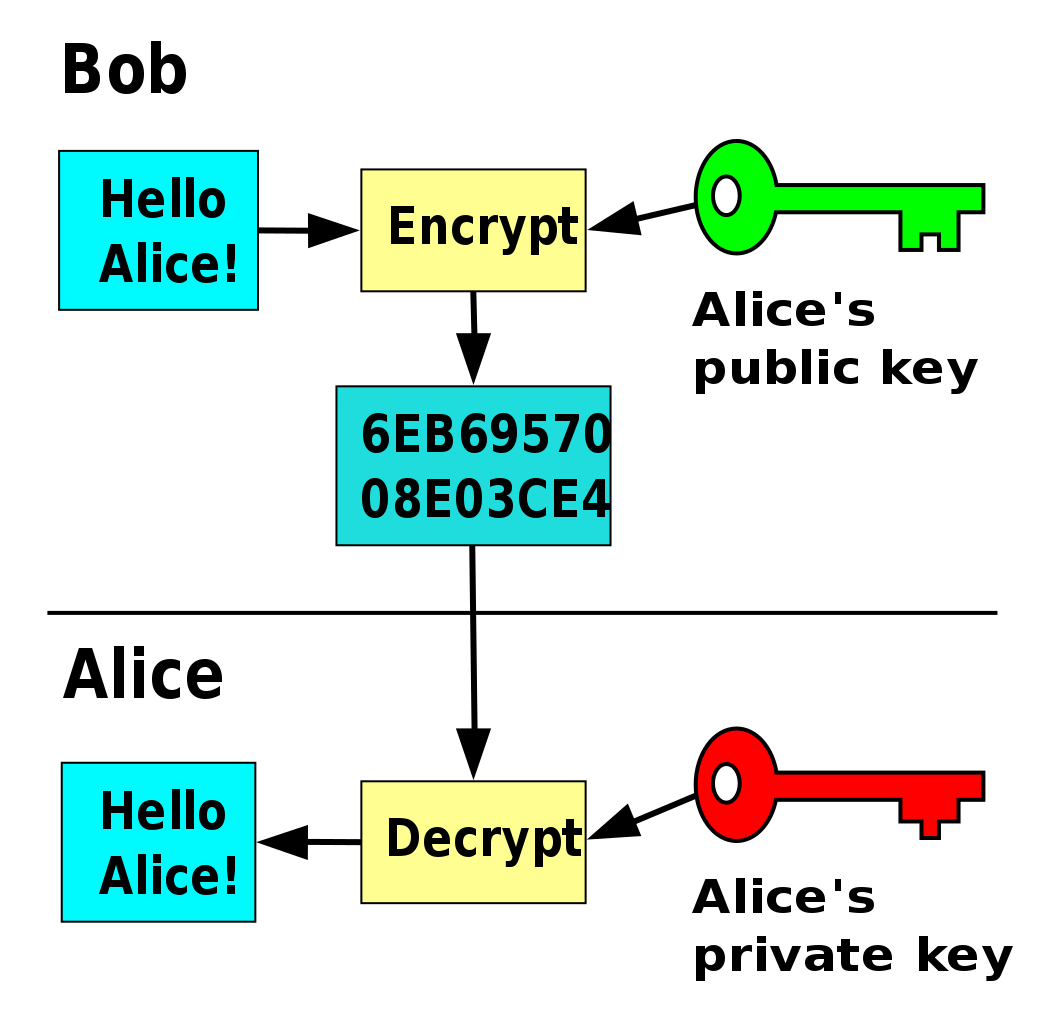
\includegraphics[width=3cm]{../pics/cryptography/1050px-Public_key_encryption}
		\end{figure}
	\column{0.3\textwidth}
		\centering \textbf{Hashing}
		\begin{figure}
		% https://commons.wikimedia.org/wiki/File:Cryptographic_Hash_Function.svg
		% public domain
		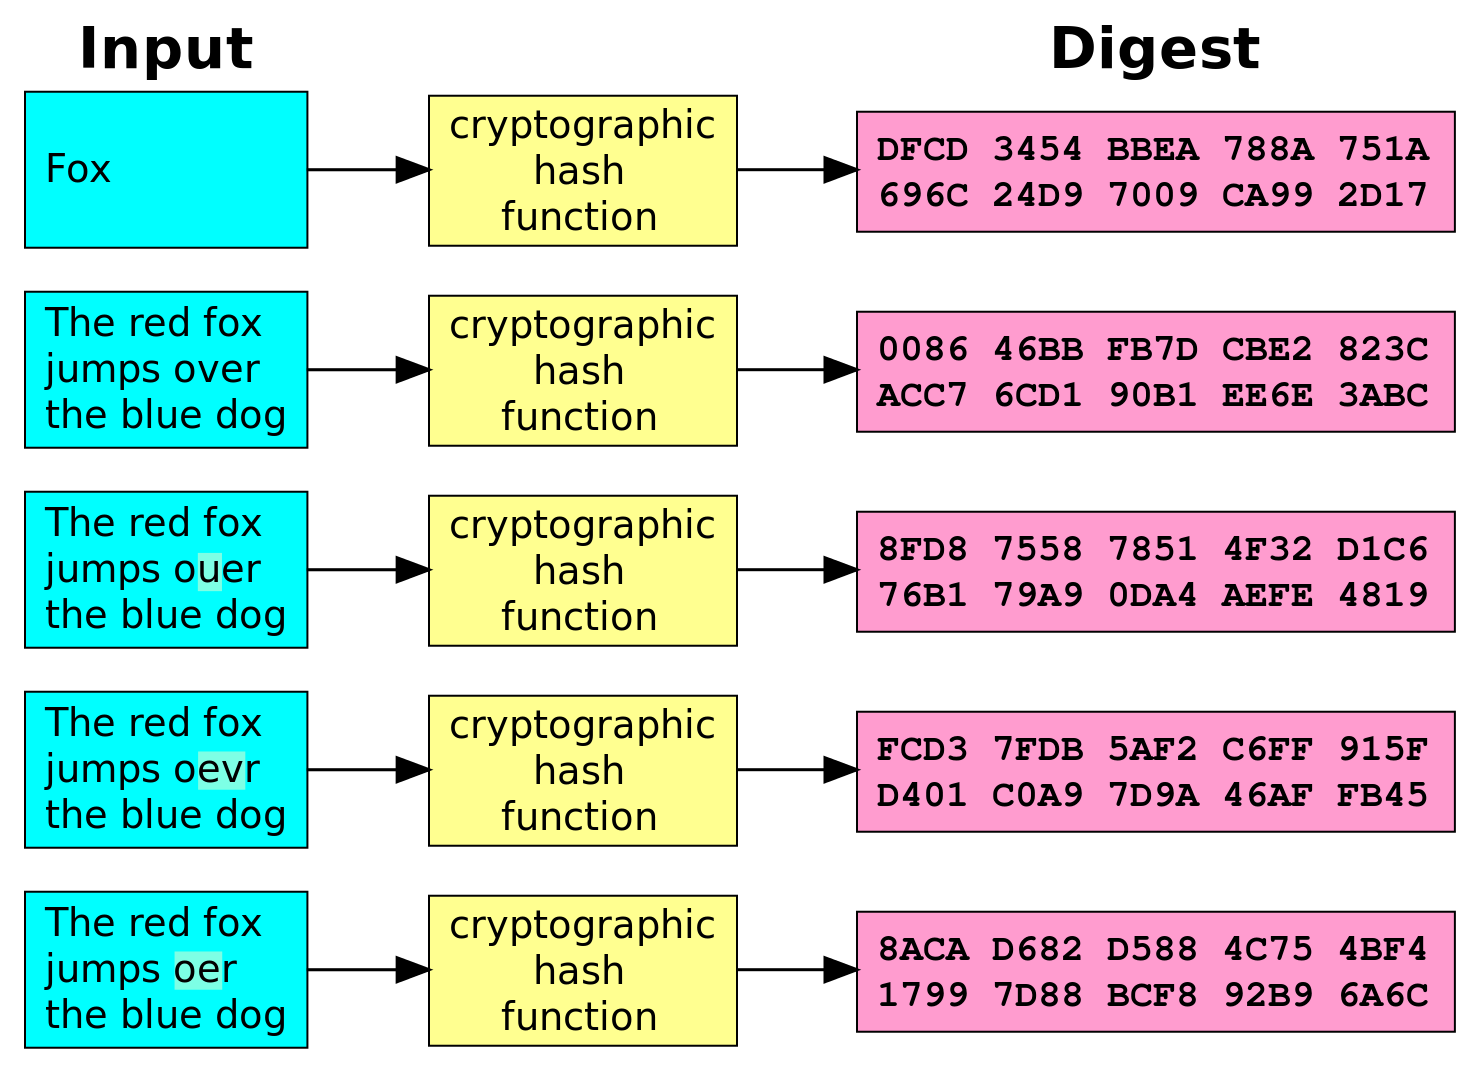
\includegraphics[width=3.6cm]{../pics/cryptography/Cryptographic_Hash_Function}
		\end{figure}
	\end{columns}
}

\frame{
	\frametitle{Where do we need more trust?}
	\begin{itemize}
		\item payments
		\pause
		\item national identity
		\pause
		\item supply chain (e.g. food: \href{https://www.ctvnews.ca/business/france-holds-trial-over-horse-meat-used-in-school-lunches-frozen-lasagna-1.4261868}{Spanghero horse meat trial}, Opioids, expensive cargos)
		\pause
		\item contracts 
		\pause
		\item \textit{real} news \& historical events (e.g. \href{https://media.consensys.net/holding-war-criminals-accountable-with-the-ethereum-blockchain-6b12471a7cdd}{bombings})
		\pause
		\item collaborative data reporting
		\item \ldots
	\end{itemize}
}

% ======================================================================================================
%                         Hands-on Introduction to Crypto, Wallets, and Custom Tokens 
% ======================================================================================================
\section{Hands-on Introduction to Crypto}
\frame{
	\frametitle{}
	\centering\Huge
	Let's try things out!
}

\frame{
	\frametitle{Install MetaMask}
	\begin{columns}
	\column{0.6\textwidth}
		Follow step by step:
		\begin{enumerate}
			\item Install the \href{https://chrome.google.com/webstore/detail/metamask/nkbihfbeogaeaoehlefnkodbefgpgknn}{Chrome/Chromium extension} 
			\item Watch the \href{https://www.youtube.com/watch?v=6Gf\_kRE4MJU}{intro on Youtube}
			\item Create an account 
			\item Switch to the Ropsten Testnet (top-right in MetaMask) 
			\item Fill your account with Ether from \url{https://faucet.metamask.io}
		\end{enumerate}
	\column{0.4\textwidth}
		\begin{figure}
			
\includegraphics[width=3cm]{../pics/ethereum/metamask-logo}
			\captionsetup{justification=centering}
			\caption*{\url{https://metamask.io}}
		\end{figure}
	\end{columns}
}

\frame{
	\frametitle{Request Ether from the faucet (on the Ropsten network)}
	\framesubtitle{Do it several times; then donate 1 ether to the faucet}
	\begin{figure}
		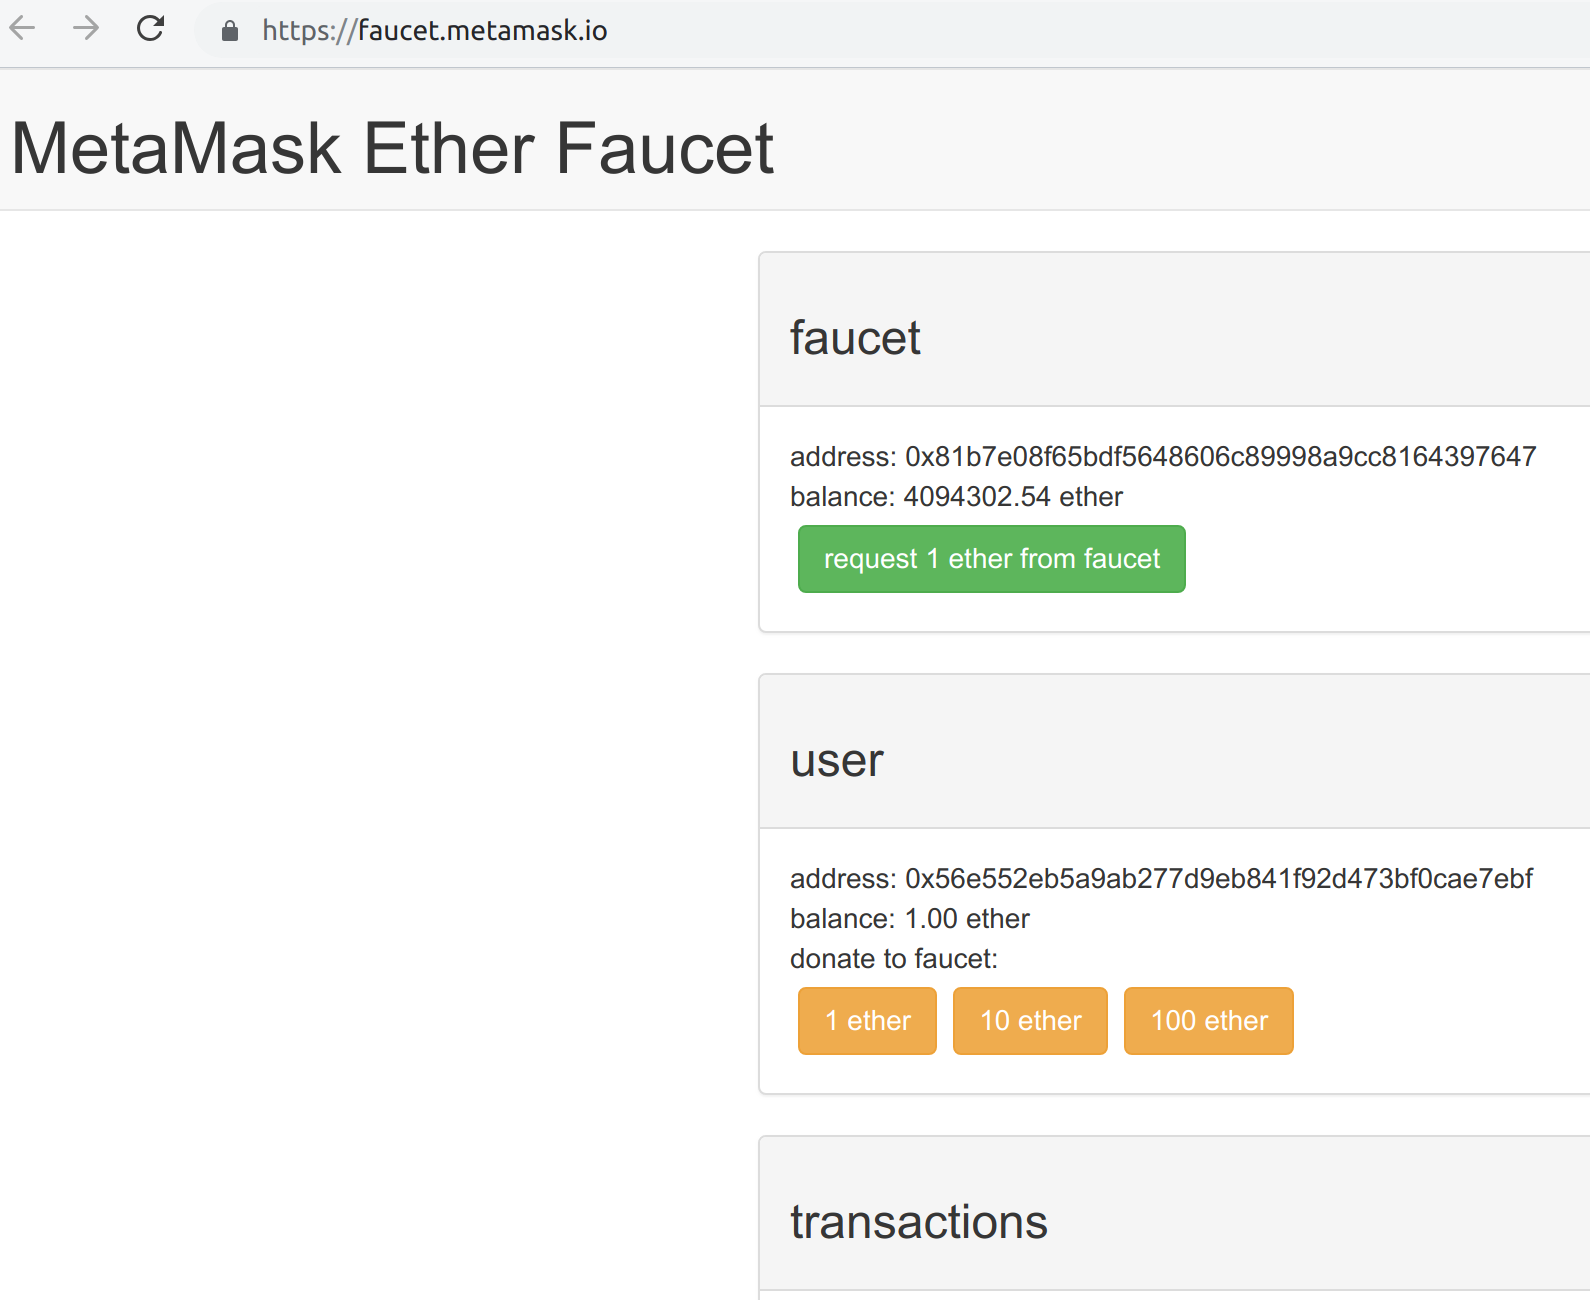
\includegraphics[width=10cm]{../pics/ethereum/faucet-ropsten}
	\end{figure}
}

\frame{
	\frametitle{Check the transaction on Metamask}
	\framesubtitle{Click on the transaction for a detailed view}
	\begin{figure}
		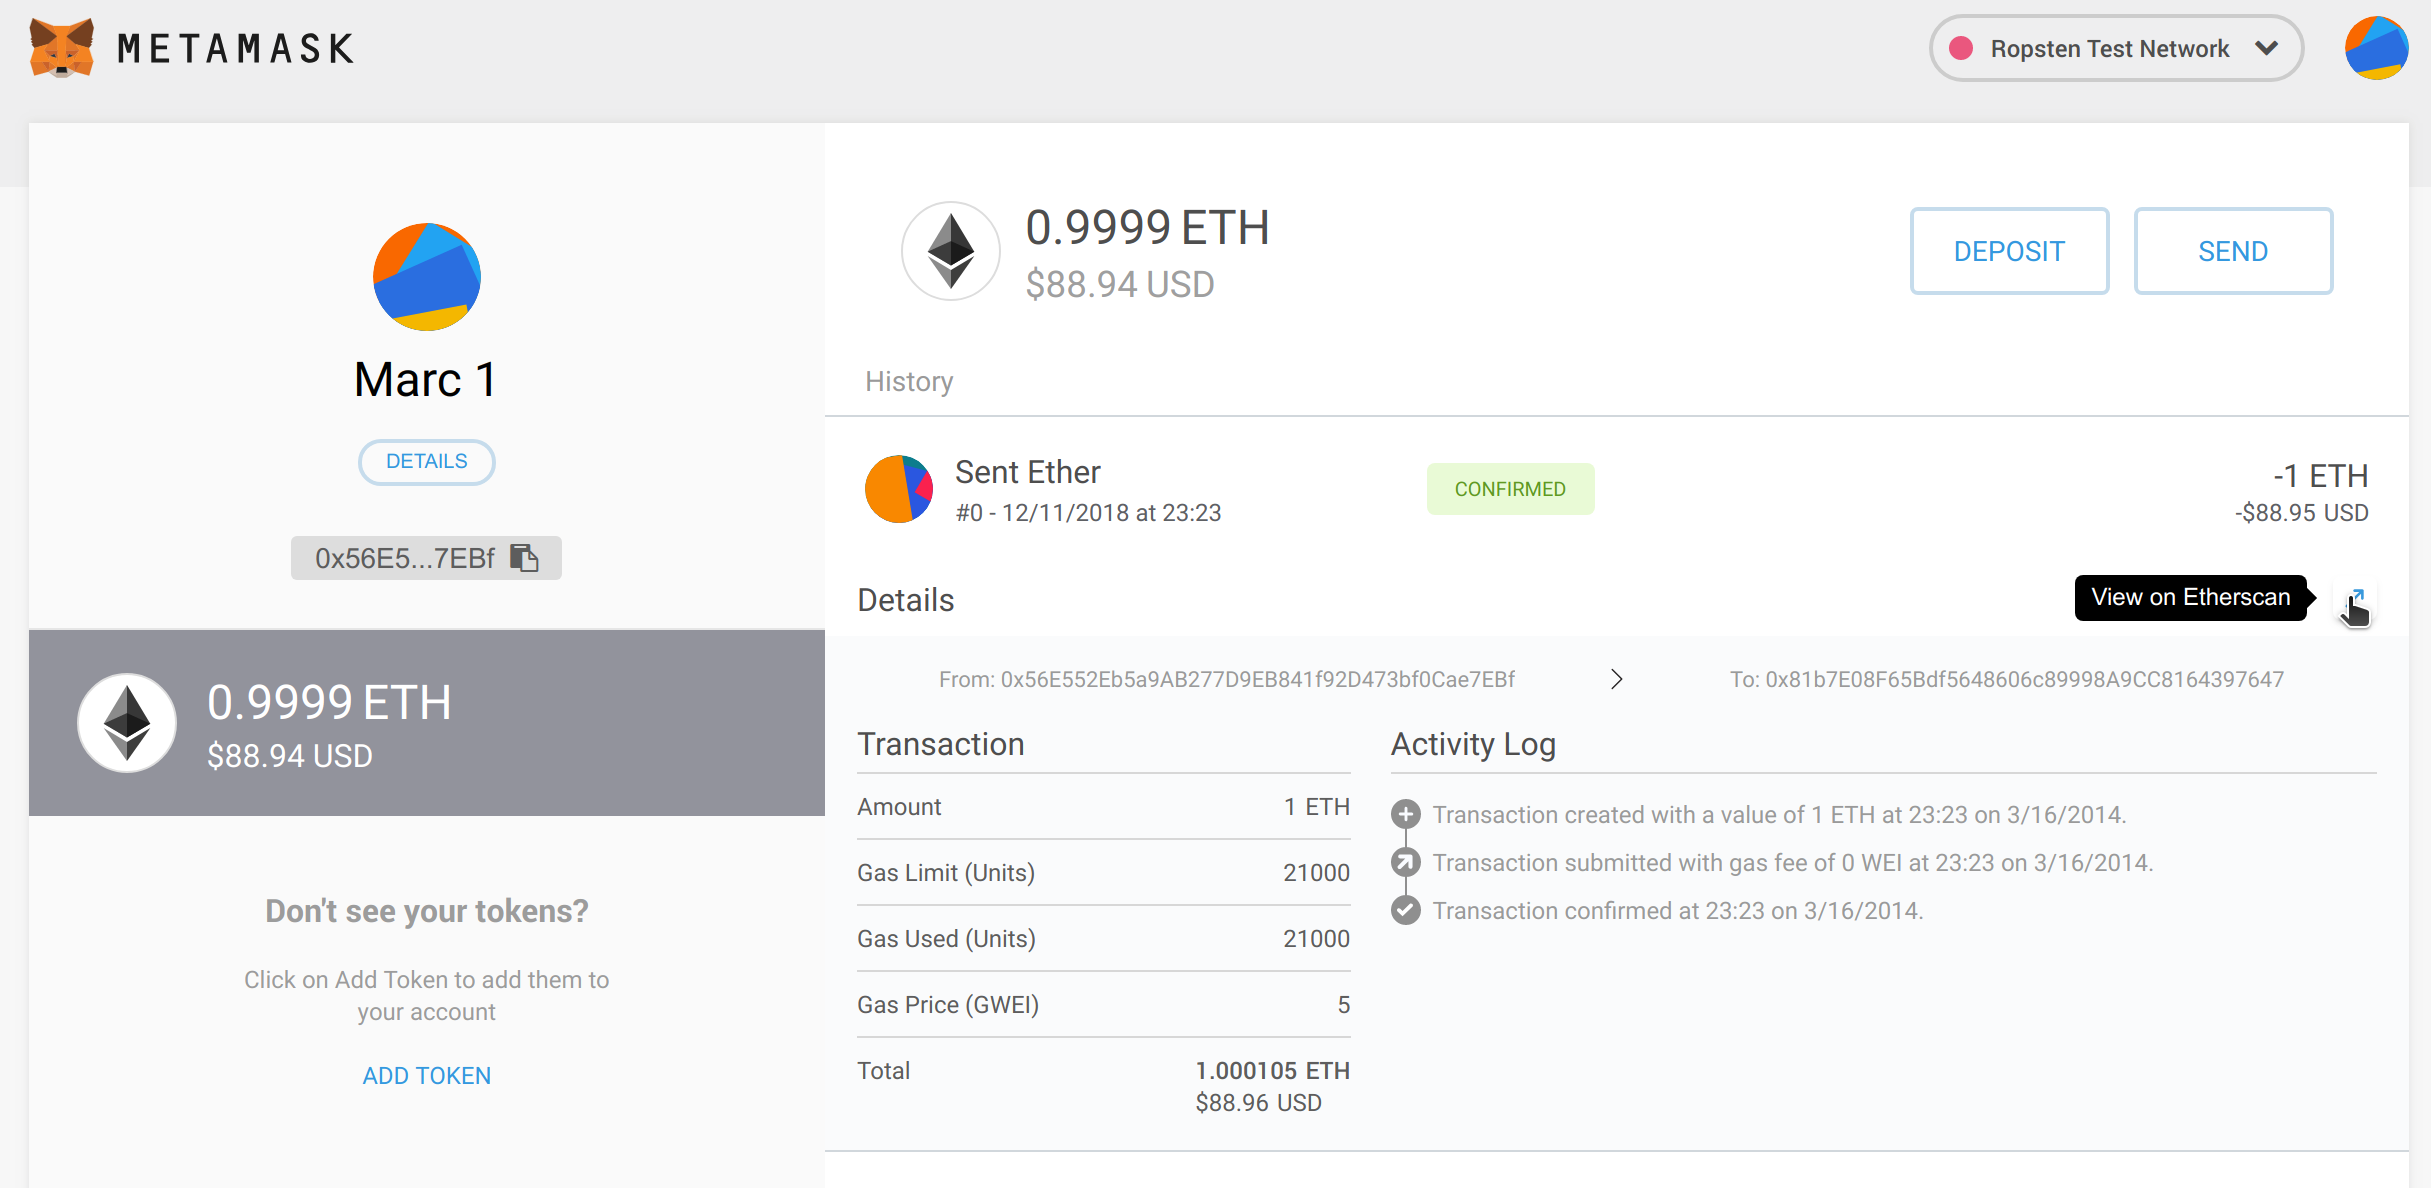
\includegraphics[width=10cm]{../pics/ethereum/metamask-tx-pane-2018}
	\end{figure}
}

\frame{
	\frametitle{Check the transaction on Etherscan}
	\begin{figure}
		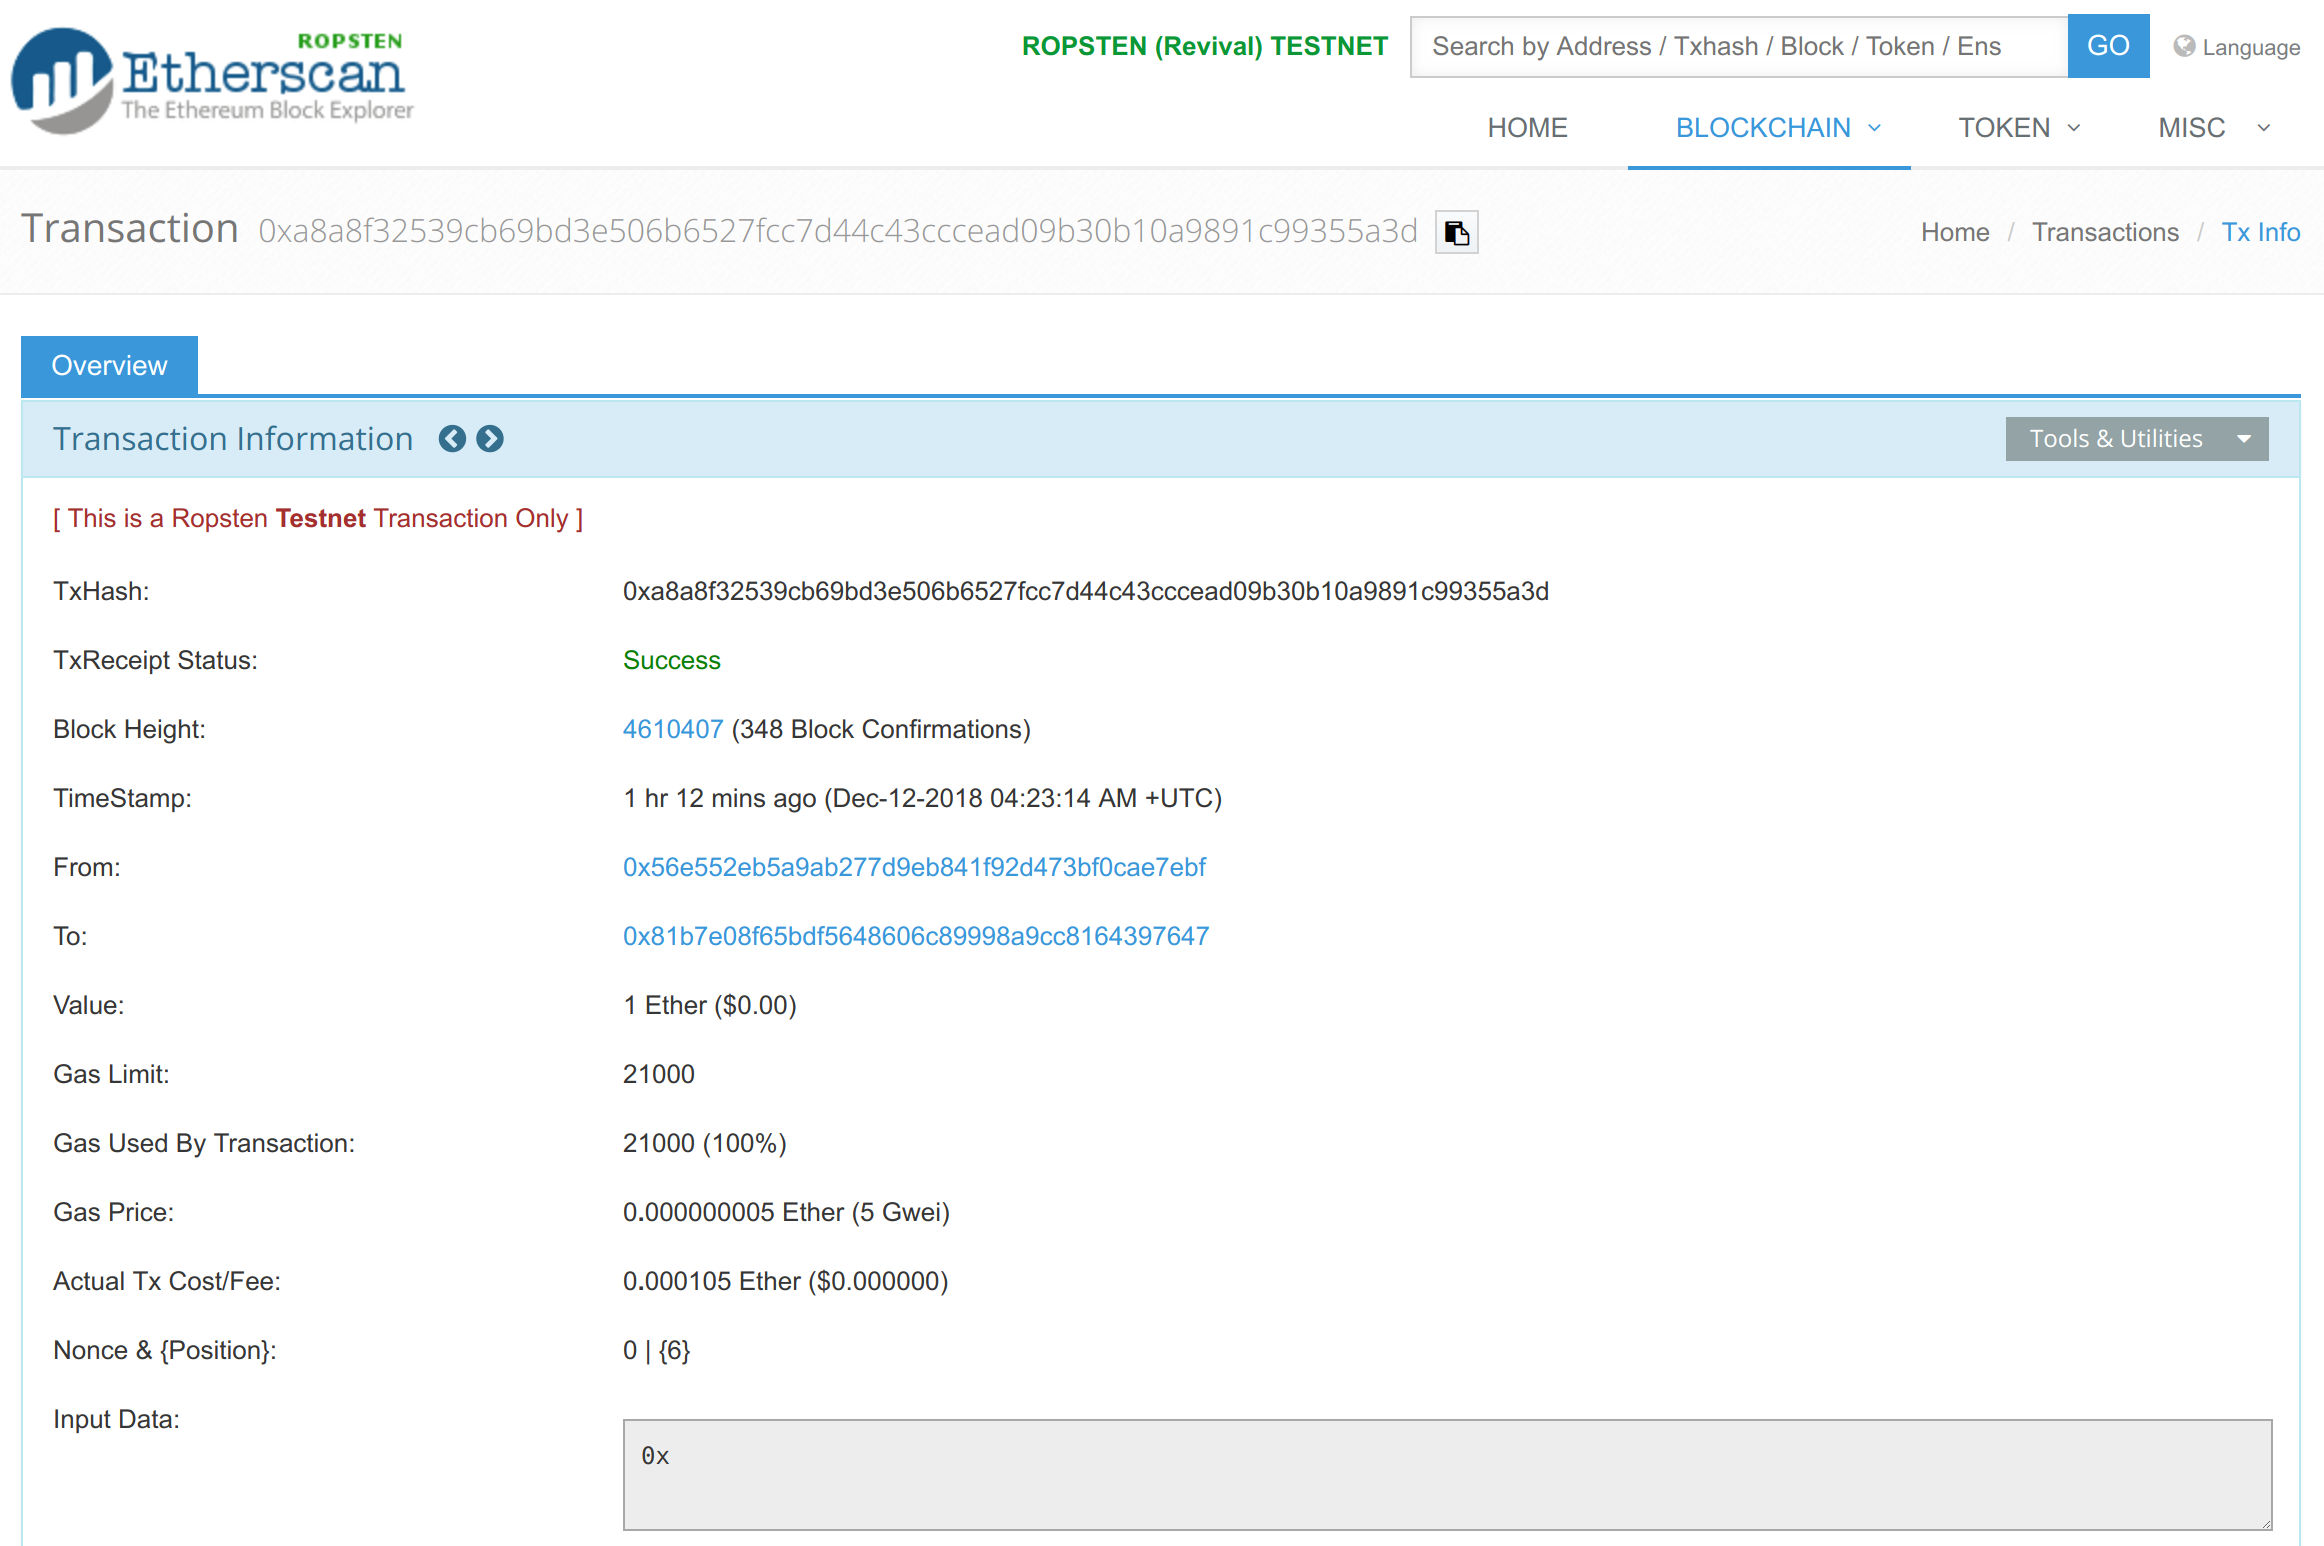
\includegraphics[width=10.9cm]{../pics/ethereum/etherscan-tx-example2}
	\end{figure}
}

\frame{
	\frametitle{A note about gas price}
	\framesubtitle{\url{https://ethgasstation.info}}
	\begin{figure}
		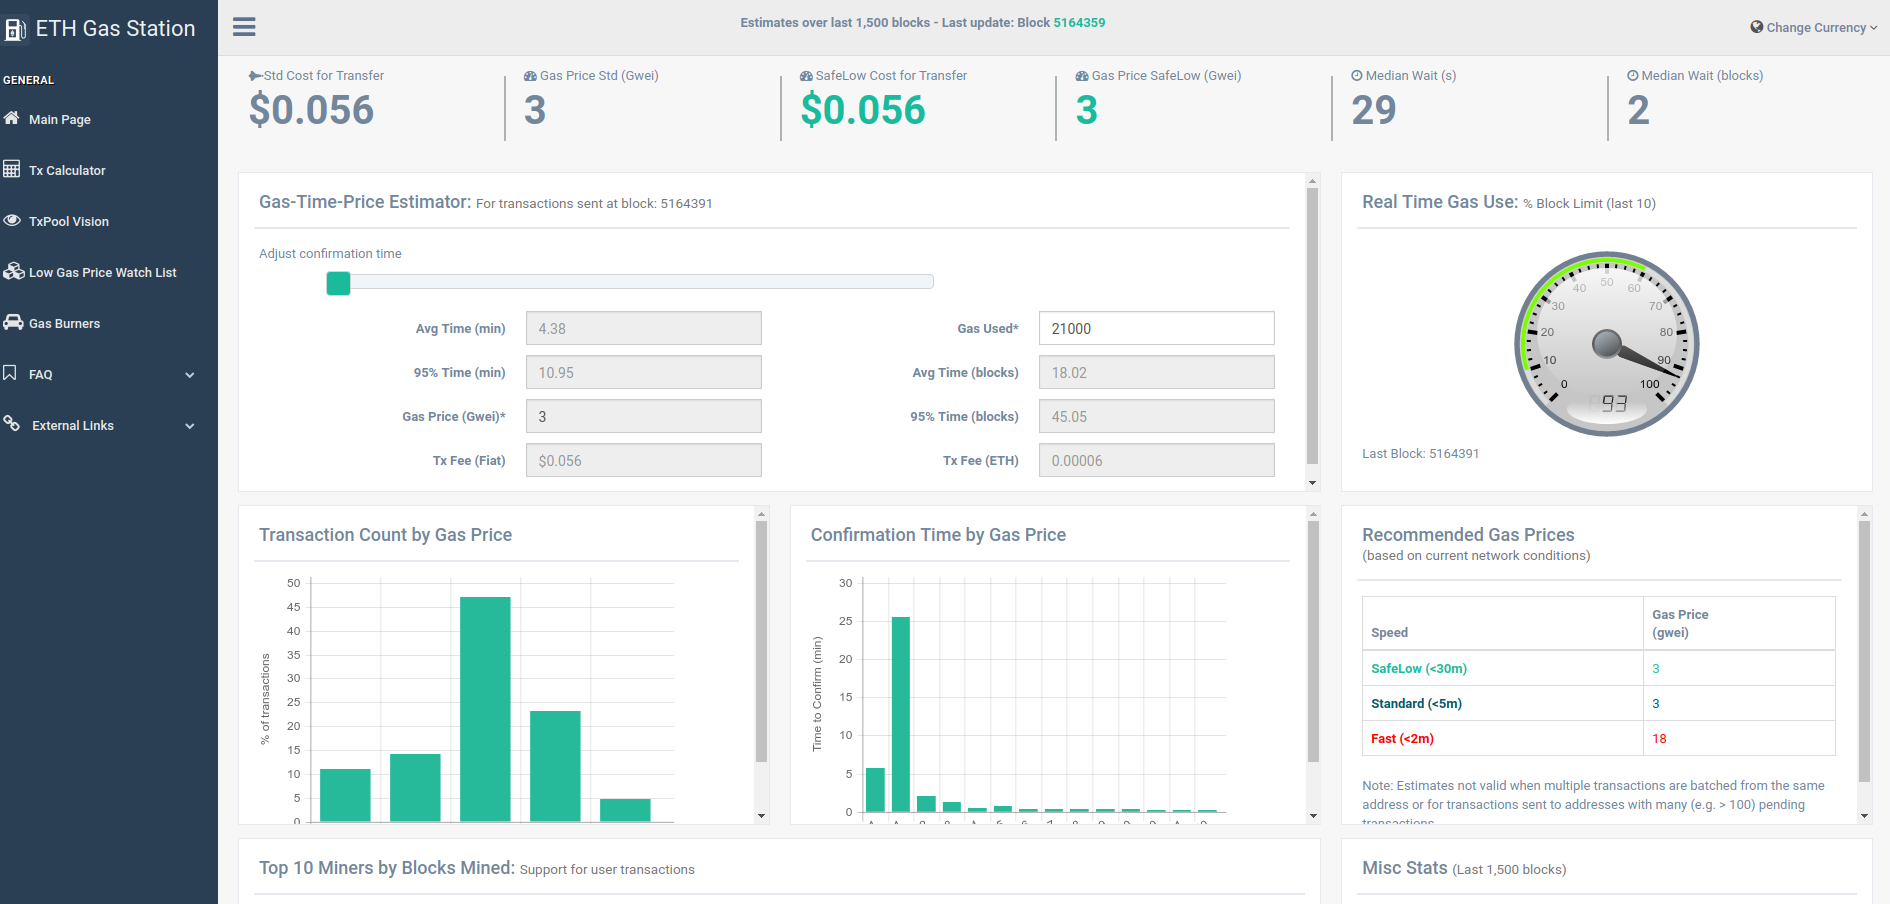
\includegraphics[width=11.5cm]{../pics/ethereum/ethgasstation}
	\end{figure}
}

\frame{
	\frametitle{Price of (real) ether: ETH}
	\framesubtitle{More information: \url{https://www.tradingview.com/symbols/ETHUSD/}}
	\begin{figure}
		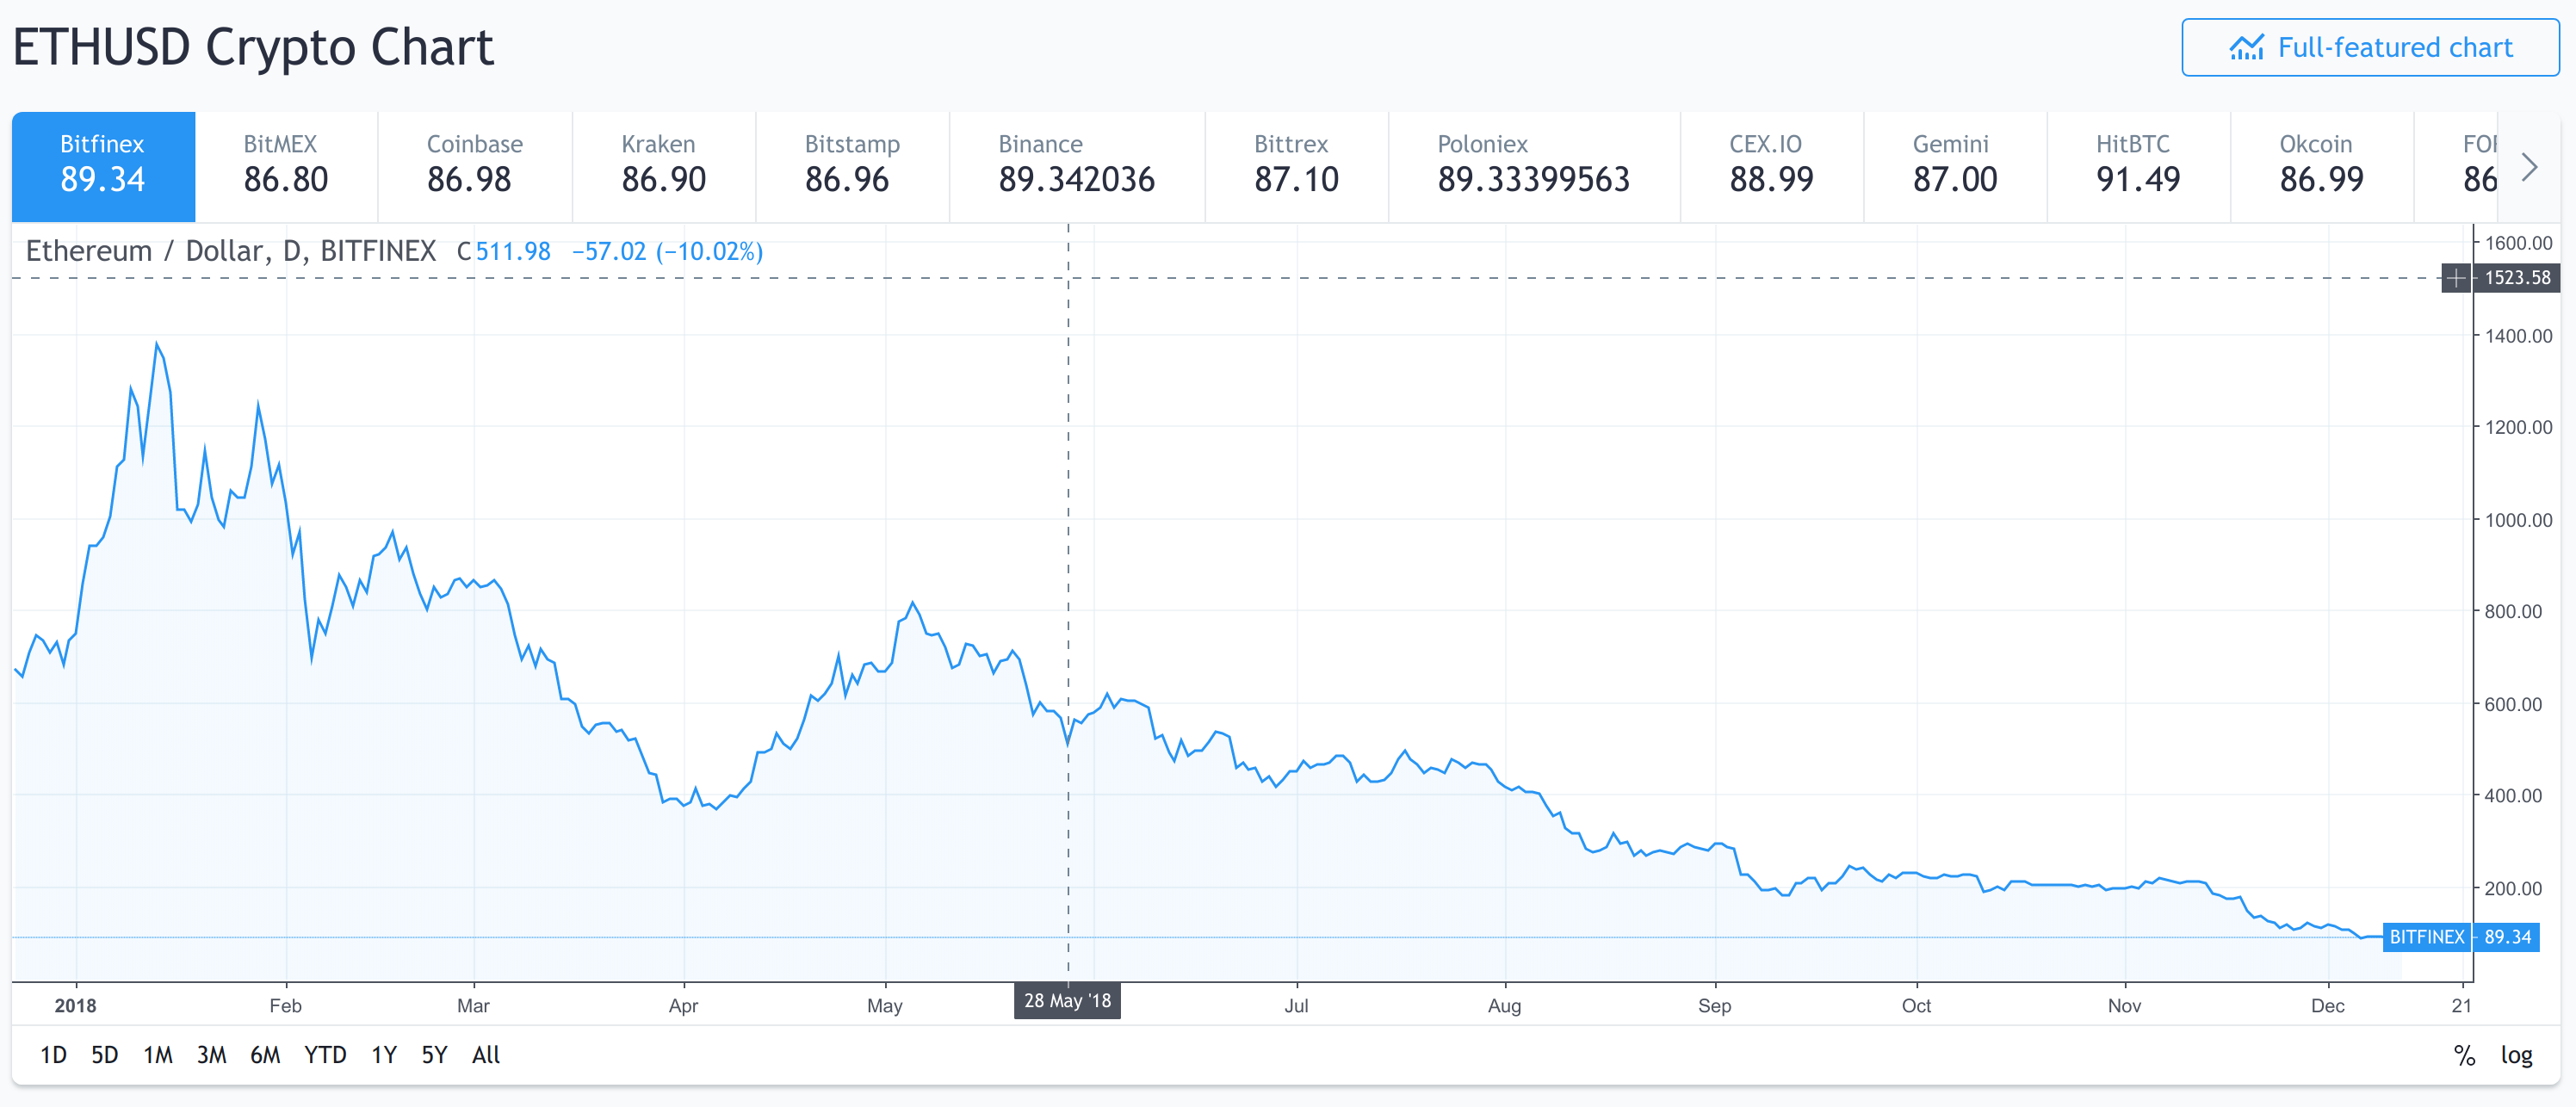
\includegraphics[width=11.5cm]{../pics/ethereum/ETH-USD-2018-12-12}
	\end{figure}
}

\frame{
	\frametitle{Wallets}
	\framesubtitle{More information: \url{https://blockgeeks.com/guides/cryptocurrency-wallet-guide/}}
	\begin{figure}
		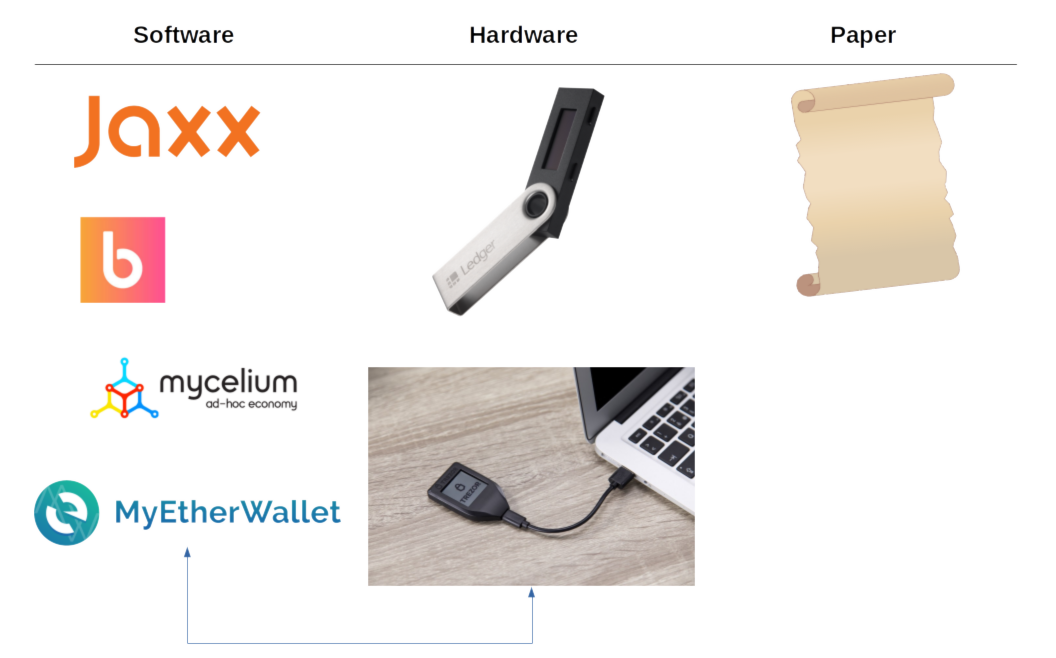
\includegraphics[width=11.5cm]{../pics/ethereum/wallets}
	\end{figure}
}

\frame{
	\frametitle{Exchanges}
	\begin{enumerate}
		\item Centralized Exchanges (Coinbase, Quadriga, ...)
		\item Decentralized Exchanges
	\end{enumerate}
}

\frame{
	\frametitle{ATMs}
	\framesubtitle{More information: \url{https://coinatmradar.com/country/38/bitcoin-atm-canada/}}
	\begin{figure}
		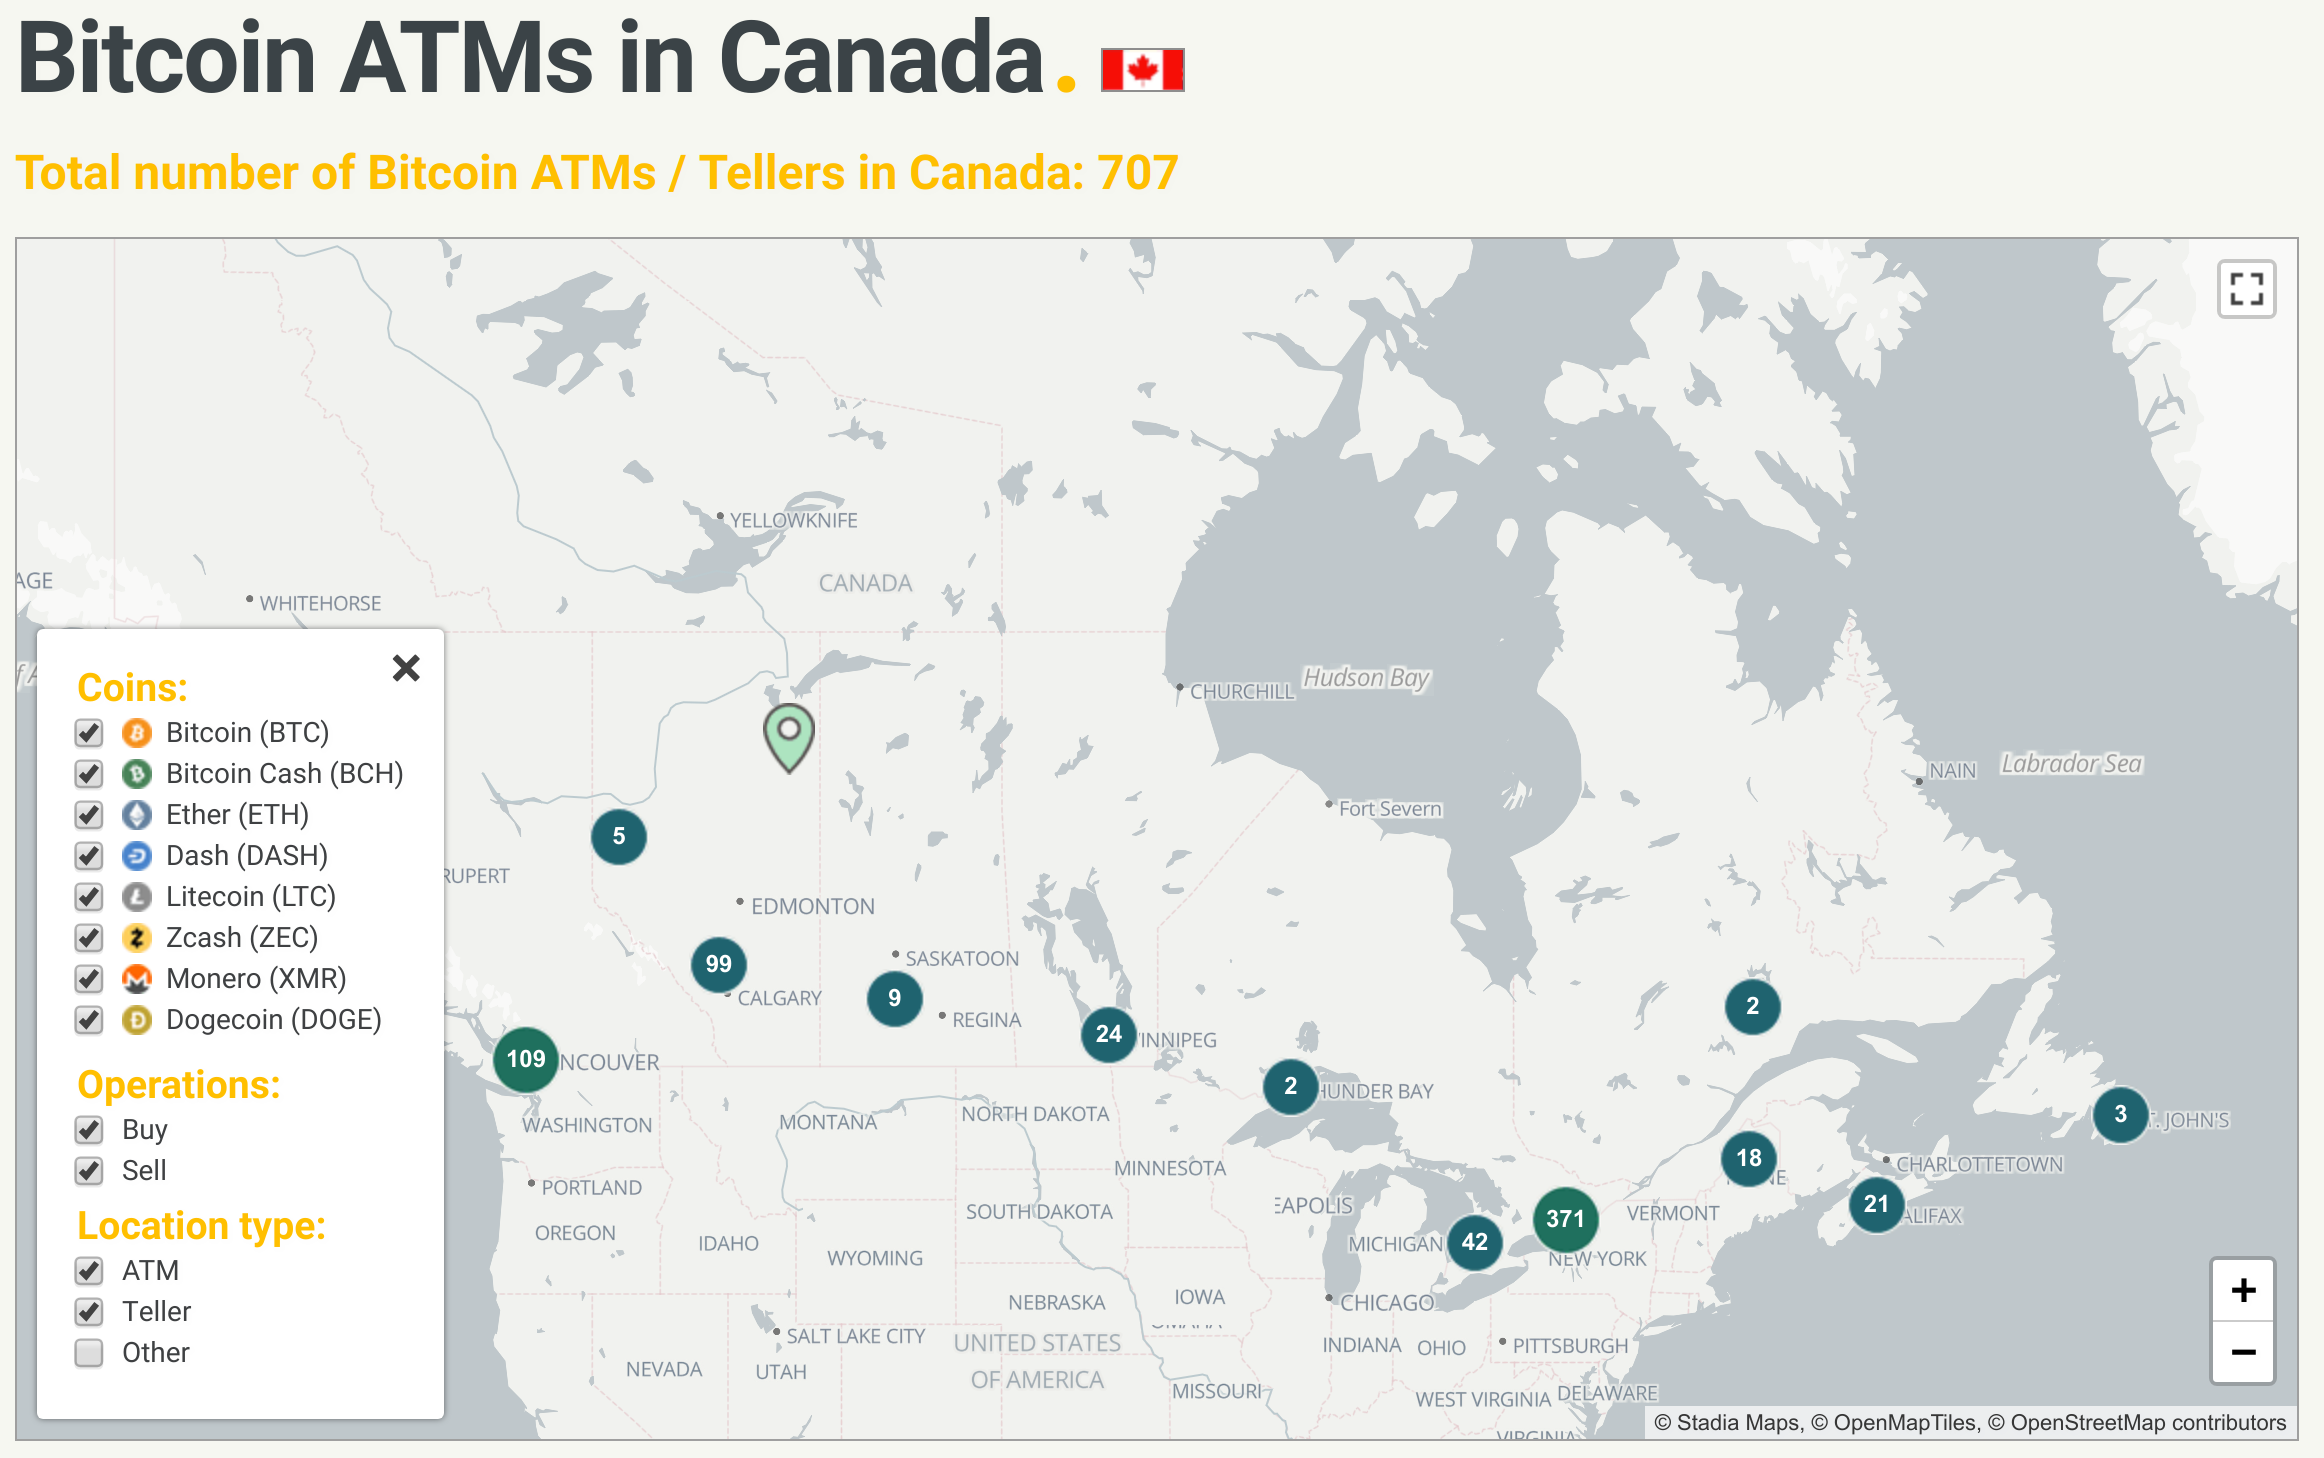
\includegraphics[width=10cm]{../pics/ethereum/bitcoin-atms-canada-2019-01}
	\end{figure}
}

\frame{
	\frametitle{ATMs}
	\framesubtitle{More information: \url{https://coinatmradar.com/country/38/bitcoin-atm-canada/}}
	\begin{figure}
		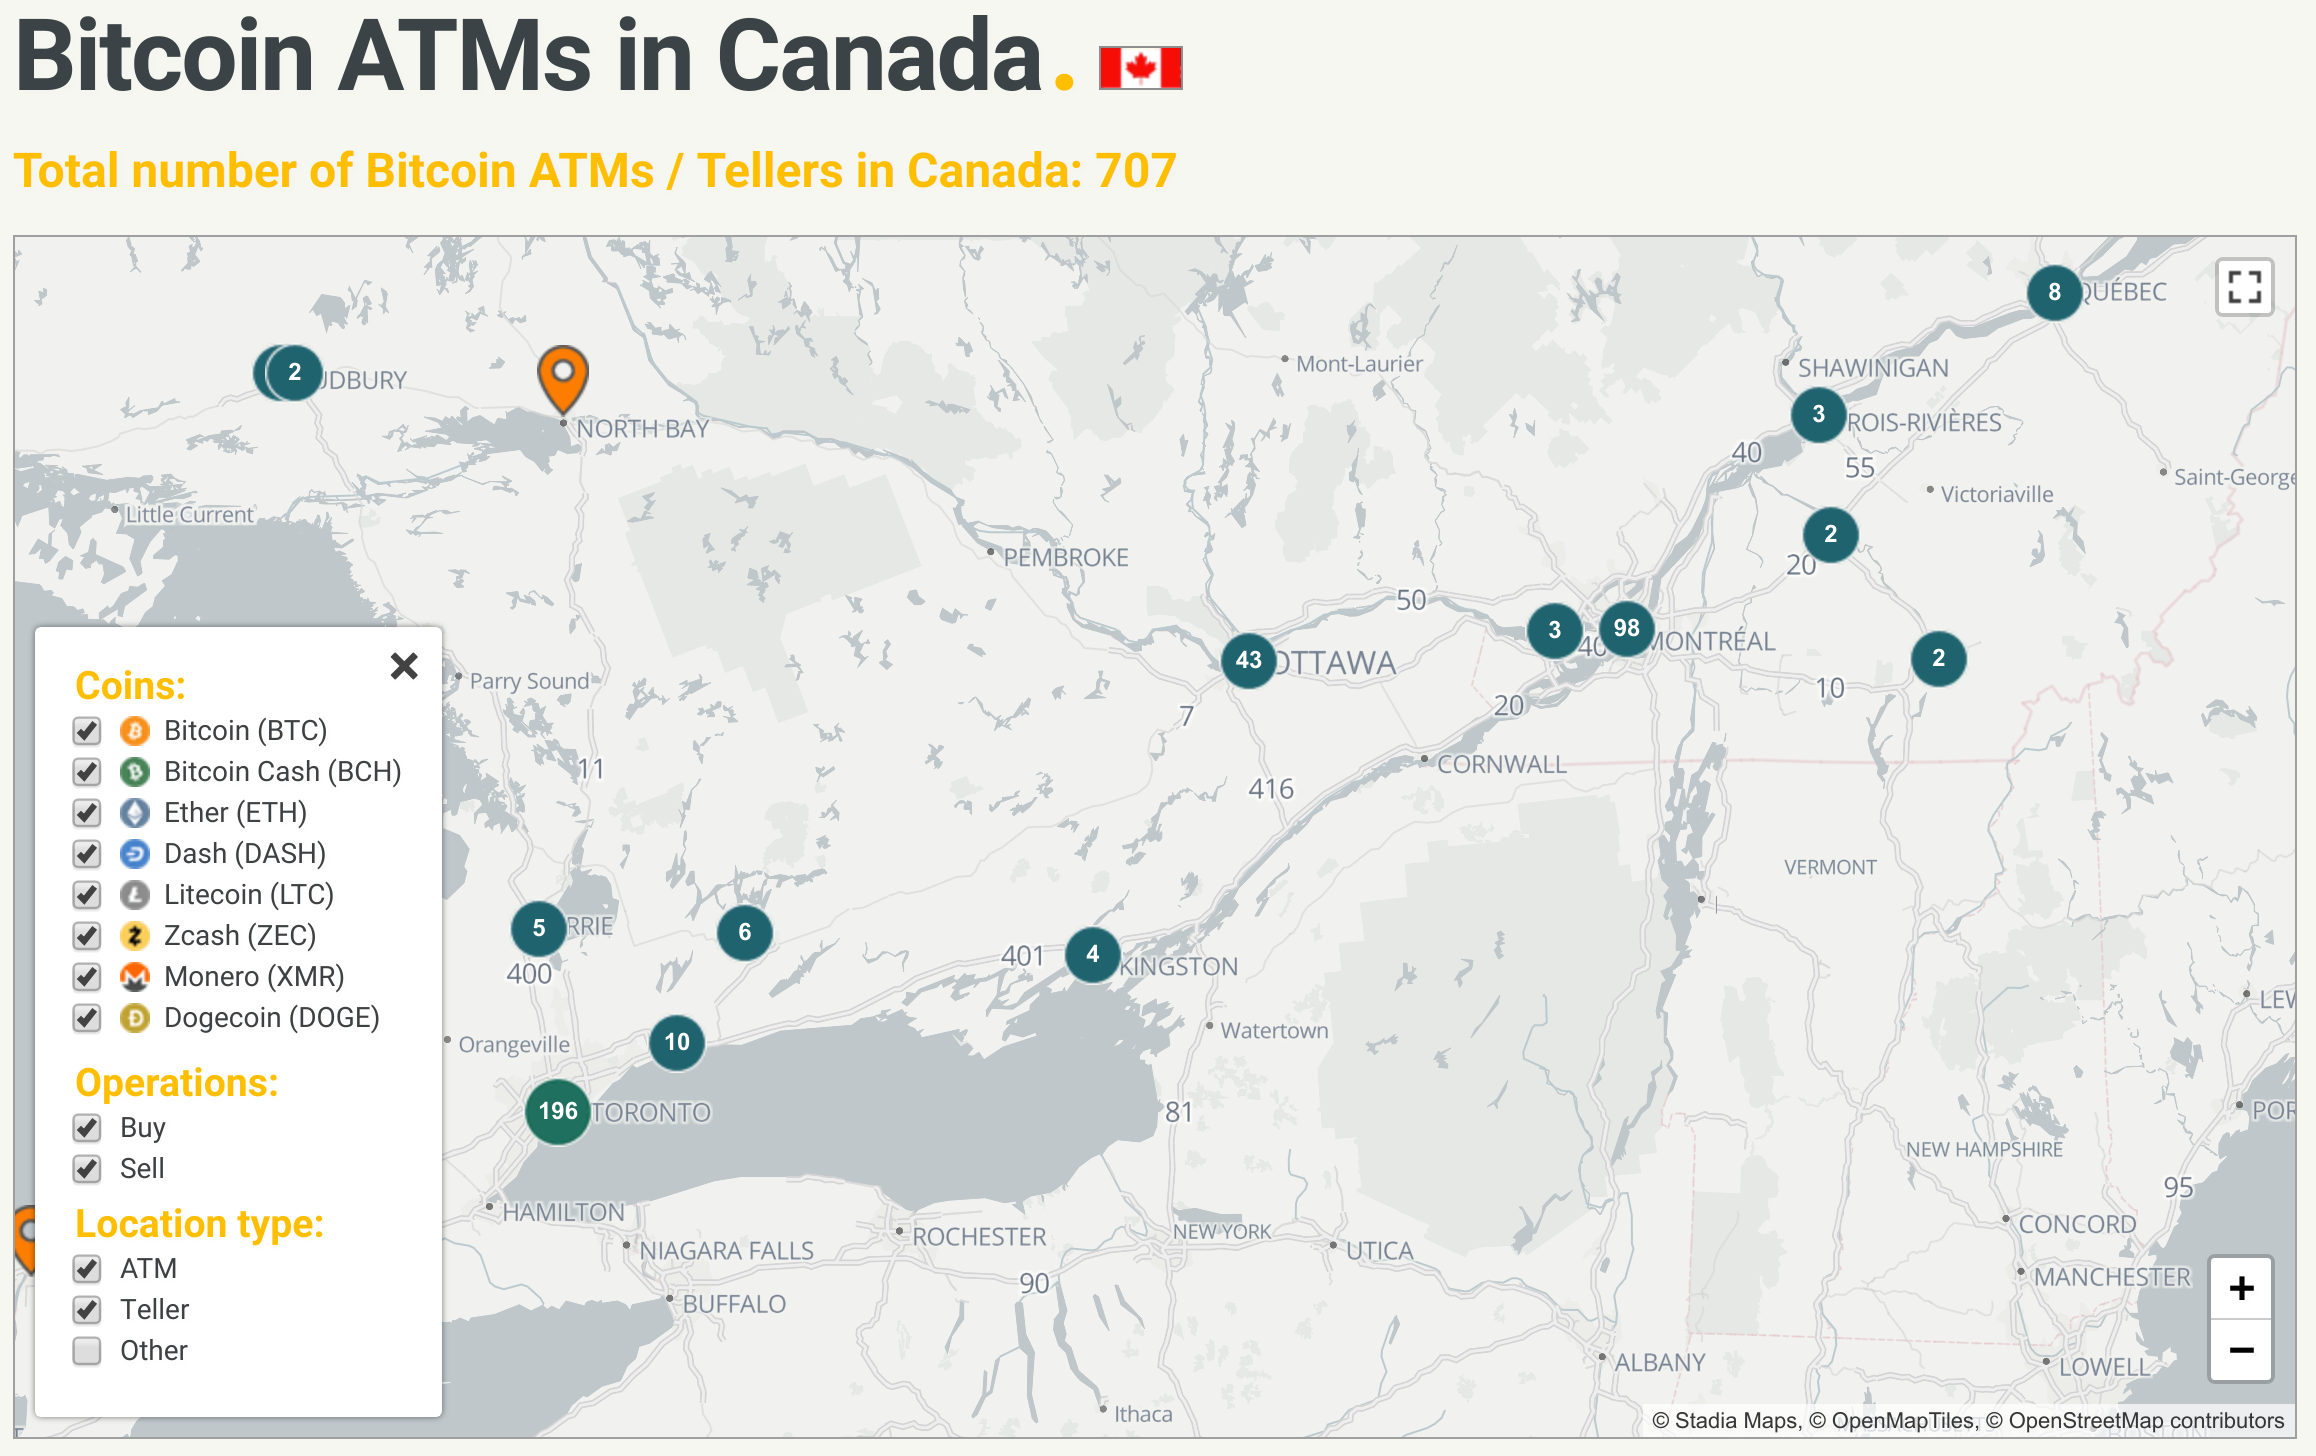
\includegraphics[width=10cm]{../pics/ethereum/bitcoin-atms-ontario-quebec-2019-01}
	\end{figure}
}

\frame{
	\frametitle{Other crypto-assets}
	\framesubtitle{More information: \url{https://www.tradingview.com/markets/cryptocurrencies/prices-all/}}
	\begin{figure}
		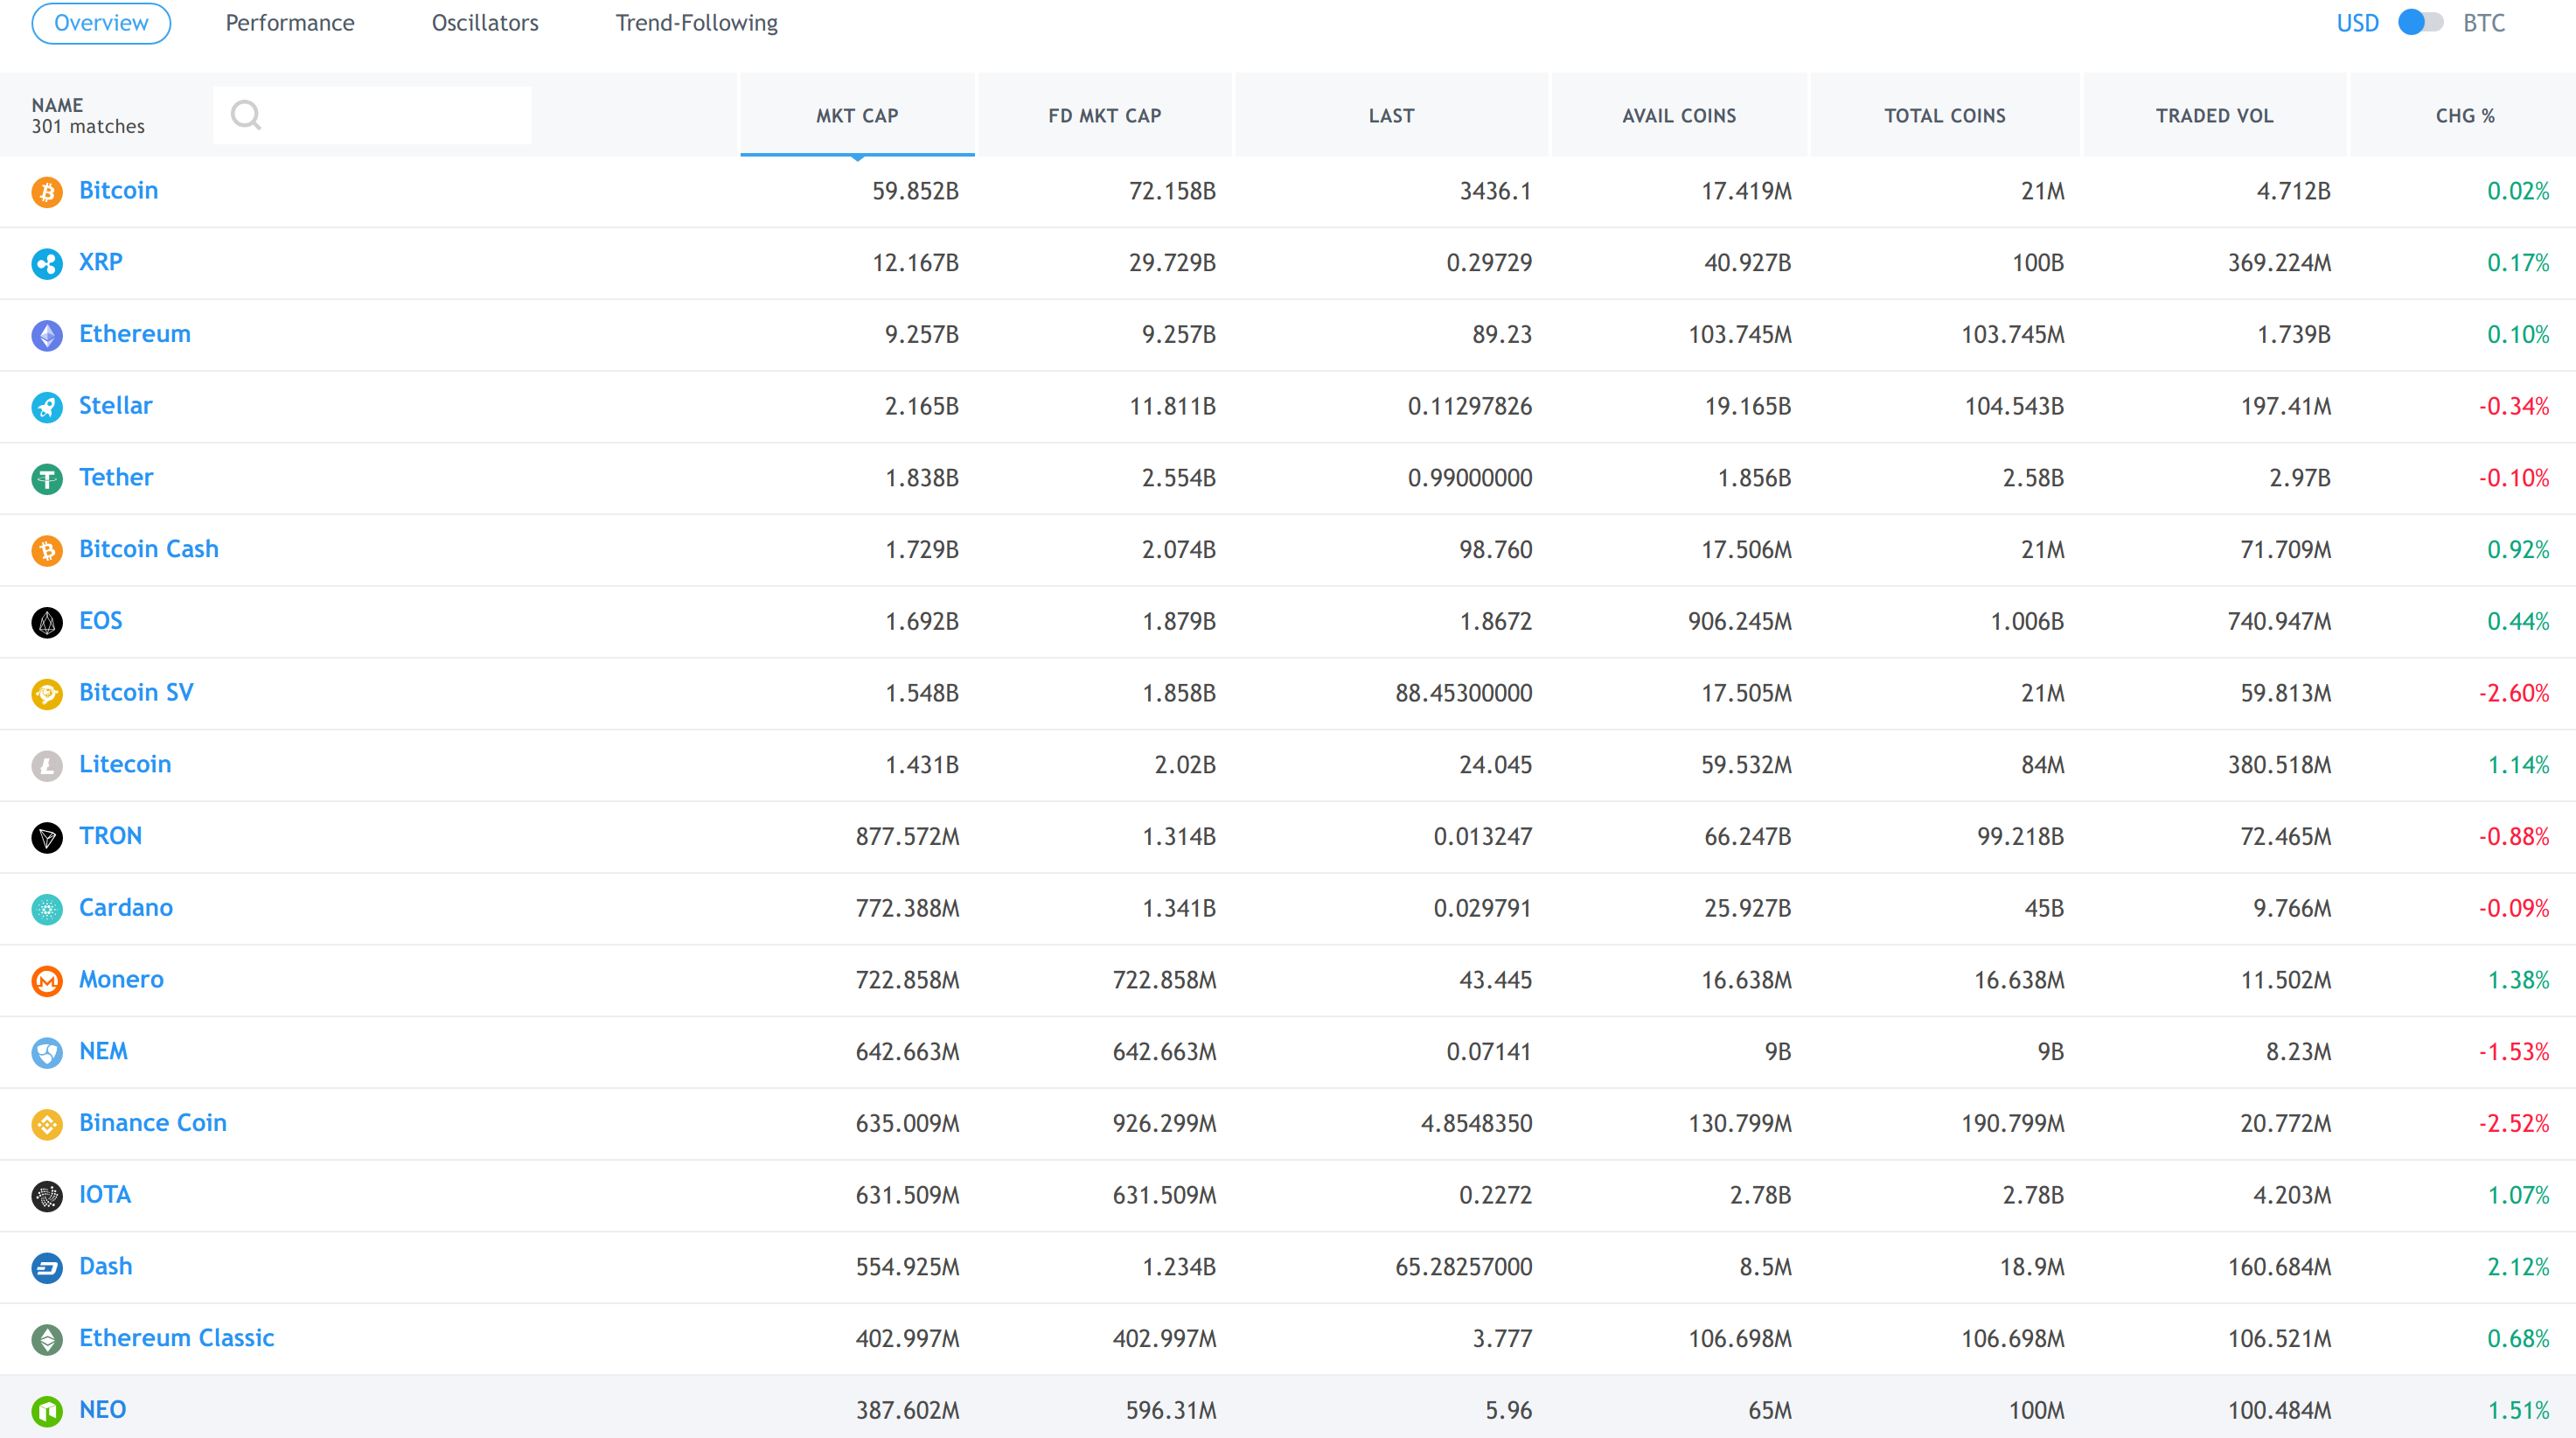
\includegraphics[width=10cm]{../pics/ethereum/coinslist-2018}
	\end{figure}
}


\frame{
	\centering\Large{Thank you!}\\
	\vspace{2em}
	{\footnotesize
		Email: \href{mailto:marc@metameshgroup.com}{marc@metameshgroup.com}\\
		Twitter: \href{https://twitter.com/marclijour}{@marclijour}\\
		\href{https://www.metameshgroup.com}{www.metameshgroup.com}
	}
}
\frame{
	\frametitle{References}
	% keyword refers to bib file: references-KEYWORD.bib, and to the Tex file: section-KEYWORD.tex  
	\printbibliography 
}
\end{document}

